\documentclass{article}
\usepackage[utf8x]{inputenc}
\title{Machine Learning - ISLR}
\author{Nico Disch }
\date{Spring 2019}
%%%TODO: UNSET LATER
\usepackage{natbib}
\usepackage{graphicx}
\usepackage{hyperref}
\usepackage{xcolor}
\usepackage{amsmath,amssymb,mathtools}
\usepackage{fullpage}

\newcommand{\cV}{\mathcal{V}}
\newcommand{\cU}{\mathcal{U}}
\newcommand{\cA}{\mathcal{A}}
\newcommand{\cM}{\mathcal{M}}
\newcommand{\cD}{\mathcal{D}}
\newcommand{\cE}{\mathcal{E}}
\newcommand{\cL}{\mathcal{L}}
\newcommand{\cJ}{\mathcal{J}}
\newcommand{\cP}{\mathcal{P}}
\newcommand{\cF}{\mathcal{F}}
\newcommand{\cH}{\mathcal{H}}
\newcommand{\cS}{\mathcal{S}}
\newcommand{\C}{\mathbb{C}}
\newcommand{\bH}{\mathbb{H}}
\newcommand{\bL}{\mathbb{L}}
\newcommand{\E}{\mathbb{E}}
\newcommand{\R}{\mathbb{R}}
\newcommand{\F}{\mathbb{F}}
\newcommand{\V}{\mathbb{V}}
\newcommand{\N}{\mathbb{N}}
\newcommand{\bP}{\mathbb{P}} % \P is used by the system



\begin{document}
\maketitle
\newpage
\tableofcontents
\newpage


\section{Introduction}
First  we might want to motivate the whole approach to machine learning. As the name suggests, we want to teach our machine to learn and maybe even predict data. Obviously this is a quite a broad topic. Hence we have several algorithms for different applications of interpretation.

\begin{figure}[ht]
    \centering
    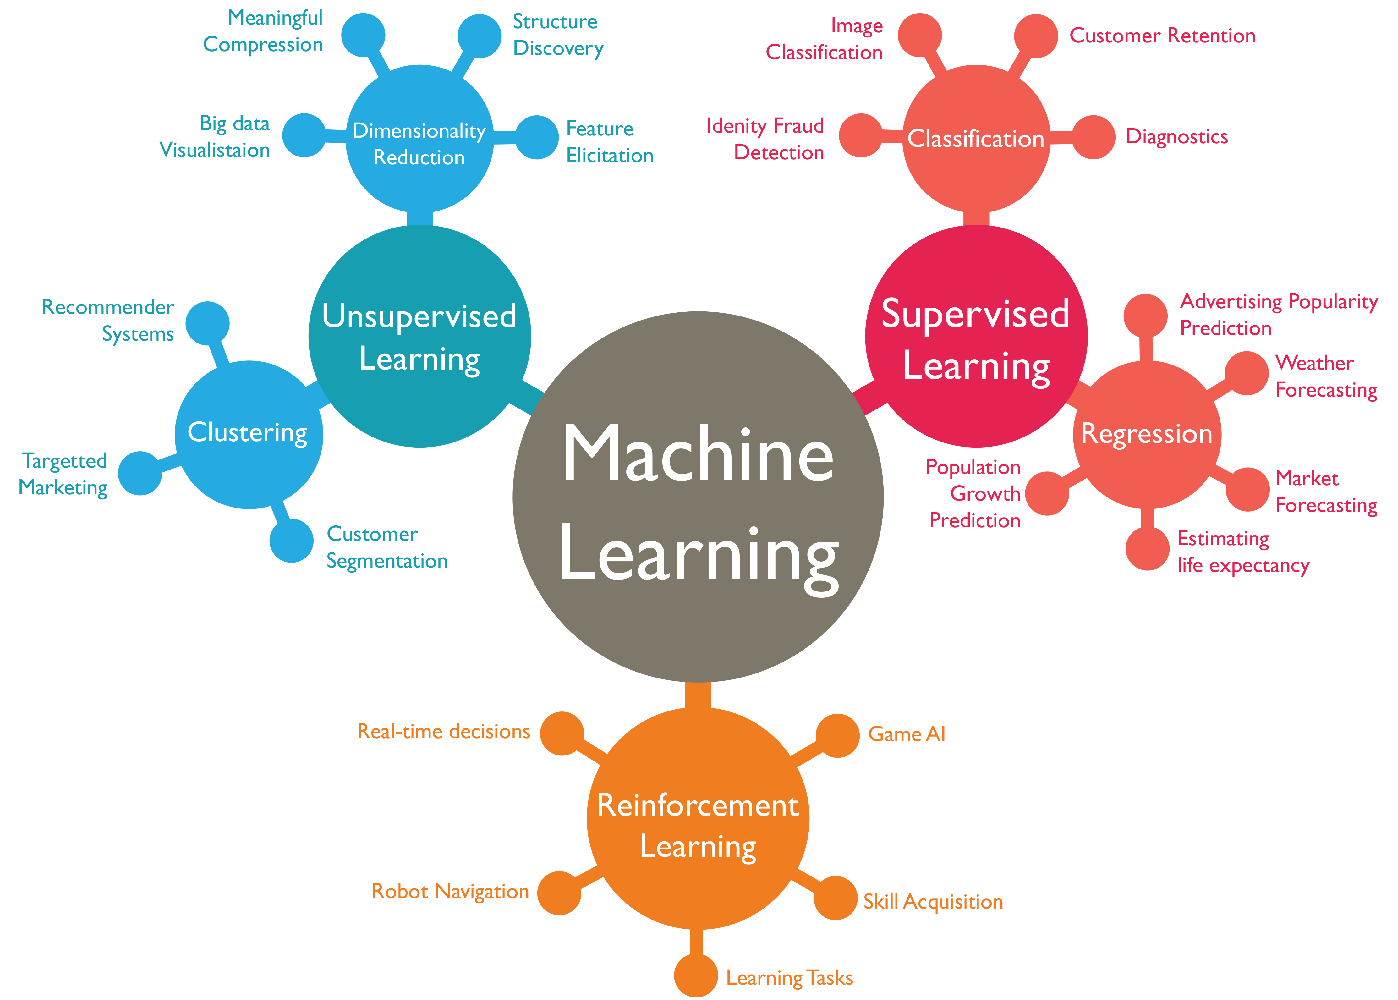
\includegraphics[width=\textwidth]{machine_learning.png}
    \caption{Basics overview of the topics in machine learning.}
    \label{fig_ml_overview_introduction}
\end{figure}

\par

For this reason all topics which use data can use machine learning. So, essentially most of science and industry.
Machine learning itself is more of an tool than a topic itself. Yet proper knowledge of that subject improves the value of it. This causes also a slight problem. Because many applications differ so much, there are so many different algorithms. Also in general it is impossible to say which parameters are good for which problem. We have to find this out for every new problem we have. With a big usability comes a lot of fine tuning. 



\par
In the following chapter we explain some more basics of the topic. Also we will follow up with some simple example.


\newpage


\section{Statistical Learning}

\subsection{Example for Statistical Learning}

To motivate statistical learning, let us consider following example:
We have a data-set for advertising, and we wish to know how advertising is onnected to sales. In this example we have TV $X_1$, Radio$X_2$ and Newspaper$X_3$, so what we want to know is the sale $Y$. So we assume that the sale is correlated to advertisement, i.e.
$$Y = f(X) + \epsilon$$

%TODO: INSERT PICTURE
%%![The correlation between advertising and sales](2.1_sales.pdf){width=1500px,height=1000px}
\begin{figure}[ht]
    \centering
    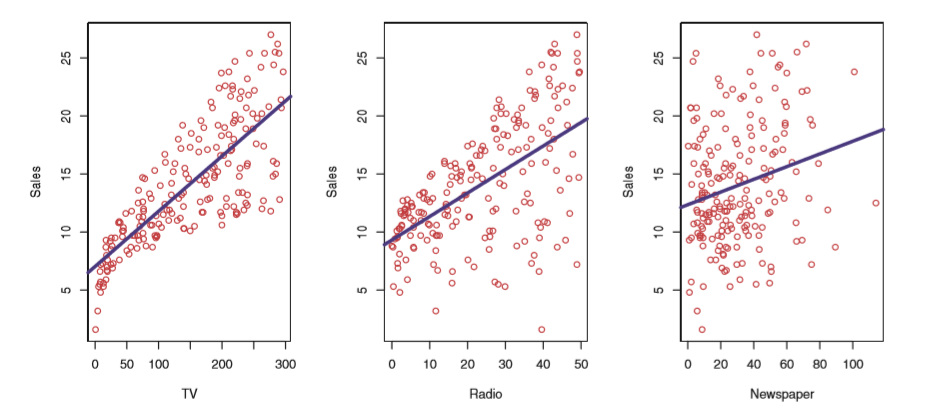
\includegraphics[width=\textwidth]{Sales_2_1.png}
    \caption{Example for Regression}
    \label{fig:sales_example_lin_reg}
\end{figure}


In this figure, you see the example of advertising, and the resulting amount of sales. 

\textit{"Machine learning (ML) is the scientific study of algorithms and statistical models that computer systems use to effectively perform a specific task without using explicit instructions, relying on models and inference instead"} -(Wikipedia).

\subsubsection{Supervised versus Unsupervised}

As mentioned, supervised learning has $i\in[1,n]$ predictor measurements $x_i$, and and associated response $y_i$. For that we want to fit a model, such that we can predict future measurements, or a better understanding between the predictors and its response.  
\par
Unsupervised learning is the situation, where we have the $x_i$ measurements, but $\mathbb{no}$ output $y_i$. Therefore we cannot fit a regression model. But still we can try to find the relation between observations and variables. An example for that is cluster analysis, where we try to find relative clustering between observations. \par

Problems that have quantitative results, i.e. numerical values, can be analysed using regression. Qualitative problems,i.e. discreet results as in Groups in a medical study, can be analysed using cluster models.  

of course we can use a regression model to examine a cluster model. If we approximate $f$ as a $\Theta$-Heaviside function, which is essentially a step function, we can transform our problem. It is even mentioned in the book, that for higher dimensions our cluster method a problem has with the high dimensionality. In higher dimensions we run into the problem that even points on a cube with length of edges $1$ distance from each other with $\sqrt(N)$ (in $N$ dimensions). Since the approach with KNN needs a proximity of measurements we either have to reduce the problem or use another algorithm.

\subsubsection{ model quality}
In order to measure how "good" our model is, we need a method to compare the prediction to the data-set. A very commonly used measure is the *mean squared error (MSE)*, which is given by the following formula:

\begin{equation}
MSE = \frac{1}{n} \sum _{i=1}^{n} (y_i - \hat{f}(x_i))^2
\end{equation}

Here $\hat{f}(x_i)$ is the prediction that $\hat f$ gives for the $i$th prediction. Thus the MSE gets lower the better our predicted $f$ is. Furthermore it is normed by $\frac{1}{n}$, such that we can compare data-sets with different sizes. \par
An important distinction has to be made: 

\subsubsection{Bias Variance Trade-Off}
The $U$-shape for the MSE curves for different flexibilities comes from the Bias Variance Trade-Off. The \textit{expected test MSE} is the average MSE over a huge set of training sets.

\begin{equation}
{E(y_0-\hat{f}(x_0))^2 = Var(\hat{f}(x_0)) + [Bias(\hat{f}(x_0))]^2 + Var(\epsilon)}
\end{equation}

\begin{align*}
E(y_0-\hat{f}(x_0))^2 &= E[(f+\epsilon - \hat{f} + E[\hat{f}] - E[\hat{f}])^2] \\
&\quad simplifying \\
&= E[(f-E[\hat{f}])^2] + E[\epsilon ^2] +E[(E[\hat{f}]-\hat{f})^2]\\
&+ \underbrace{ 2 E[(f-E[\hat{f}])\epsilon] + 2E[\epsilon( E[\hat{f}]-\hat{f})] + 2E[(E[\hat{f}]-\hat{f})(f-E[\hat{f}])]}_{vanishes} \\
&\text{where we used that $E(\epsilon)=0$ and that f and $\hat{f}$ are not correlated}\\
&= \underbrace{ (f - E[\hat{f}])^2 }_{Bias\quad of \quad \hat{f}} + E[\epsilon ^2] + \underbrace{ E[(E[\hat{f}]-\hat{f})^2]}_{Var[\hat{f}]} \\
& = Bias[\hat{f}]^2 + Var[y] + Var[\hat{f}] 
\end{align*}


This trade-off can be explained in the following way;
The Variance increase with increased flexibility comes from the fact that if you over-fit the data, the result will be horrific for other training set. This means the fit is \textbf{only} good for \textbf{this} data-set. But because different data-sets have different randomly spread points it varies between different sets.
On the other hand if you have a very small flexibility, e.g. a linear approximation for a highly non-linear model, then the Bias is increased.

\subsubsection{Classification Problem }

The classification setting is useful if we do not want to use a numerical value, i.e. classes as "gender" or "marital status". So now we have a training observation $x_i$ for $i\in [1,n]$, and qualitative observations, $y_i$. Here we cannot use the MSE, so we define another measure, called the error rate. 

\begin{equation}
\frac{1}{n} \sum _{i=1}^{n}I(y_i\neq \hat y _i )
\end{equation}
Because this error rate is dependent on the specific training set, we average over several training sets, refer to the MSE for different training sets. One can show that the average of the error rate is minimised by using the Bayes classifier, which is a simple conditional probability. We assign a test for each predictor $x_0$ to each class $j$ for which the following is maximised. 

\subsubsection{Bayes Classifier}

\begin{equation}
\mathbb P (Y=j | X = x_0)
\end{equation}
!!find better explanation to the classifier
So we have an empirical classification, $\mathbb{if}$ we know how the data is distributed. So for example the following data-set consists of two predictors $X_0,X_1$ and two classes, i.e. orange and blue.




This is a simulated data set for an example for two classes $orange,blue$ and two predictors $X_0,X_1$. The orange background will be the area where points will be assigned to the $orange$ class, and vice versa for the blue area. The coloured points are the simulated points we measure. The violet line is where $\mathbb P (Y=j | X = x_0) = 0.5$. So any model that tries to find the $\textit{decision boundary}$ can at most be as good as the Bayes model.

\begin{figure}[ht]
    \centering
    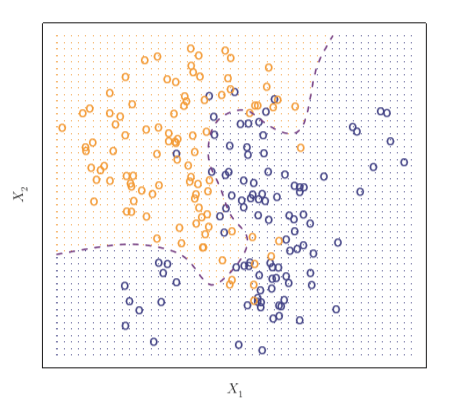
\includegraphics[height=70mm]{bayes_classifier_chapter2.png}
    \caption{The Bayes Classifier for a specific example: orange class 1, blue class 2 and purple is the classifier for $\Pr (X=x_0)=50\% $}
    \label{fig:bayes_classifier_example}
\end{figure}




\subsubsection{K Nearest Neighbours - KNN}

Calculating the Bayes classifier is impossible without knowing the distribution, so we use the KNN method, to approximate it, and obviously we can only hope to reach the accuracy of our Bayes model. The conditional probability is calculated the following way:


\begin{equation}
\mathbb{P} (Y=j | X = x_0) = \frac{1}{K}\sum _{i \in \mathcal{N} _ 0} I
(y_i=j)
\end{equation}

The \textit{KNN} test identifies the $K$-nearest points of the data set towards our chosen point $x_0$. $I$ identifies if the neighbour $i \in \mathcal{N} _ 0$ is at the value $j$, giving out a $1$, if not a $0$. So the total probability is between $0$ and $1$, as it should be. Similar to the linear regression we can have a fit that is too rigid ($K$ is too high), or a fit that is too flexible($K$ is too low). We see that in the following example Fig.\ref{fig:KNN_high_low_compare}.

\begin{figure}[ht]
    \centering
    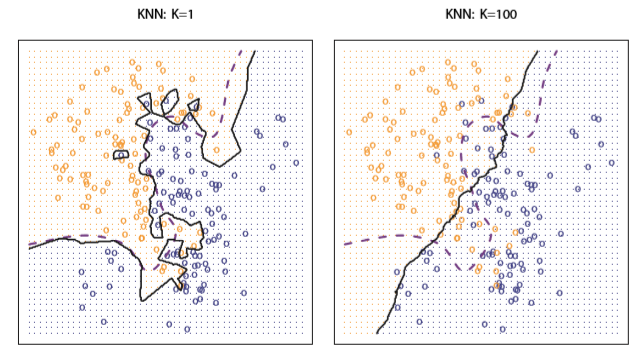
\includegraphics[width=\textwidth]{KNN_high_low.png}
    \caption{The difference between high($K=1$) and low flexibility($K=100$)}
    \label{fig:KNN_high_low_compare}
\end{figure}

\newpage

\section{Linear Regression}
\subsection{Notes}
It is essentially what the name says; We predict that our response is linearly dependent on our predictor. It doesn't have to be exactly linear, but only approximately. We have:

$$ Y \approx \beta_0 + \beta_1 X $$

In total, $\beta_0$ and $\beta_1$ are known as the model parameters. Once we used our training data, we have for the future prediction:

$$ \hat y =\hat \beta_0 + \hat \beta_1 x $$
whereby $\hat y$ is the prediction based on $X=x$.

\subsubsection{ Estimating the Coefficients}


In order to find our coefficients $\beta_0$ and $\beta_1$, we need to ``fit''
our data to the linear model. We consider the dataset $(x_i,y_i), i \in [1,n]$,
and let $\bar x$ and $ \bar y$ denote the sample means.
Let $\hat y_i =\hat \beta_0 + \hat \beta_1 x_i $, and set $e_i=y_i - \hat y _i$
as the $i$th residual. We define the $\textit{residual sum of squares}$ as
$\text{RSS} = \sum_{i=1}^n e_i^2$. Or alternatively, $\text{RSS}' = \sum_{i=1}^n
(y_i - \hat\beta_0-\hat\beta_1(x_i-\bar x))^2$, where we just shift the mean. We
want to minimize RSS,  and in order to do that we set the derivative zero
(assume that the function is concave, hence we do not need to calculate if that
is a minimum or maximum):
 \[
 \frac{d \text{RSS}}{d\hat{\beta_0}} =    2 \sum_{i=1}^n (y_i -
 \hat\beta_0-\hat\beta_1x) =0,  
\]
which implies
\[
    n\hat{\beta_0} =  \sum_{i=1}^n (y_i -\hat\beta_1x).
\]
Therefore, 
\begin{equation}\label{eq_beta_0_lin}
 \hat \beta _0 = \bar y - \hat \beta _1 \bar x.
\end{equation}

For the other parameter we have:
\begin{equation}
\hat \beta _1 = \frac{\sum_{i=1}^n(x_i-\bar x)(y_i - \bar y)}{\sum_{i=1}^n(x_i - \bar x)^2}=\frac{\text{Cov}(x,y)}{\text{Var}(x)}. 
\end{equation}
Similar to $\hat{\beta}_0$, we differentiate RSS with respect to $\hat{\beta}_1$ and set it zero again:
\[
       \frac{d \text{RSS}}{d\hat{\beta_1}}=   \sum_{i=1}^n x_i(y_i -
       \hat\beta_0-\hat\beta_1 x_i) =0,
\]
Using~\eqref{eq_beta_0_lin}, we have 
\[
  x_i(y_i -
       \hat\beta_0-\hat\beta_1 x_i) = x_iy_i - x_i\bar{x}+\hat{\beta_1}\bar{x}x_i -\hat{\beta_1}x_i^2,
     \]
     which implies that
     \[
     \hat{\beta_1}=\frac{\sum_{i=1}^n (x_iy_i-x_i \bar{x}) }{\sum_{i=1}^n (x_i^2-\bar{x}x_i) }. 
     \]
     Furthermore, since
     \[
       \sum_{i=1}^n (\bar{x}^2-\bar{x}x_i) = \sum_{i=1}^n (\bar{x}y_i-\bar{x}\bar{y})=0,
     \]
\begin{align*}
        \hat{\beta_1} & = \frac{\sum_{i=1}^n (x_iy_i-x_i \bar{x}) -\sum_{i=1}^n (\bar{x}y_i-\bar{x}\bar{y}) }{\sum_{i=1}^n (x_i^2-\bar{x}x_i) +\sum_{i=1}^n (\bar{x}^2-\bar{x}x_i) }\\
       & = \frac{\sum_{i=1}^n (x_i-\bar{x})(y_i-\bar{y})}{\sum_{i=1}^n (x_i-\bar{x})^2}=\frac{\text{Cov}(x,y)}{\text{Var}(x)}. 
\end{align*}

\subsubsection{Assess the Accuracy}
As we denoted before, our $f$, only approximates the true measurement $Y$. $Y = f(X) + \epsilon$, thus we have in the linear model:

$$ Y = \beta _0 + \beta_1 X + \epsilon$$
Since we like to wish to know $\mu$, we approximate it as the average over several measurements.The variance of $\mu$ is a know entity in statistics for normal distributed variables; $\text{Var}(\mu)=SE(\mu)^2=\frac{\sigma^2}{n}$, with $\sigma$ as the standard deviation of each $y_i$. Similarly we have that,

$$\text{Var}(\hat\beta_0)=\sigma^2 \bigg{[}  \frac{1}{n} + \frac{\bar x^2}{\sum_{i=1}^n(x_i-\bar x)^2} \bigg{]}  \quad \quad Var(\hat\beta_1)= \frac{\sigma^2}{\sum_{i=1}^n(x_i-\bar x)^2} $$
Where we have the assumption that $\epsilon_i$,error for each observation, is not correlated with $\sigma^2$, common variance, which is in reality only an approximation. In general we do not know $\sigma$, but it can be estimated from the data as the \textit{standard residual error} $RSE = \sqrt{RSS/(n-2)}$ (2 for the amount of predictors). Proof for $\hat{\beta}$:

To simplify a few things one uses the property that was established while calculating $\hat{\beta}_1$, and then we calculate $Var(\hat{\beta})$

\begin{align*}
  \sum_{i=1}^{n}(x_i-\bar{x})(y_i-\bar{y}) & = \sum_{i=1}^{n}(x_i-\bar{x})y_{i} \\
  &=\sum_{i=1}^{n}(x_i-\bar{x})(\beta_0 + \beta_1 x_i + a_i)\\ 
  \\
% <<<<<<< HEAD
%   Var(\hat{\beta}_1) & = Var\Bigg{(} \frac{\sum_{i=1}^n(x_i-\bar x)(y_i - \bar y)}{\sum_{i=1}^n(x_i - \bar x)^2}\Bigg{)}\\
% =======
  % &\text{We use this in the calculation, and substituting for the definition of}   \hat{\beta}_1 \\
  % Var(\hat{\beta}_1) & = Var\Bigg{(} \frac{\sum_{i=1}^n(x_i-\bar x)(y_i - \bar y)}{\sum_{i=1}^n(x_i - \bar x)^2}\Bigg{)}\\
  &=Var \Bigg{(} \frac{\sum_{i=1}^n(x_i-\bar x)(\beta_0 + \beta_1 x_i + a_i)}{\sum_{i=1}^n(x_i - \bar x)^2}\Bigg{)}\\ 
  & \text{only $a_i$ is a random variable, whose Var doesn't vanish}\\
  &= Var \Bigg{(} \frac{\sum_{i=1}^n(x_i-\bar x)a_i}{\sum_{i=1}^n(x_i - \bar x)^2}\Bigg{)}\\
  &\text{use quadratic property of Var and independence of variables}\\
  &=\frac{\sum_{i=1}^n(x_i - \bar x)^2 Var(a_i)}{(\sum_{i=1}^n(x_i - \bar x)^2)^2}\\\
  &=\frac{\sigma^2}{\sum_{i=1}^n(x_i - \bar x)^2}
\end{align*}

Where we defined $a_i \sim \mathcal{N}(0,\sigma^2)$ as a random variable for the random error term $\sigma_i$. For the calculation of $\hat{\beta}_0$, we use the fact that $\hat{\beta}_0 = \bar{y}-\hat{\beta}_1 \bar{x}$ and the independence between every variable.
With this we wish to calculate the \textit{Null-Hypothesis}:
We want to test whether our $\beta_1=0$ or not, because we want to know if our outcome and predictor are correlated. Therefore we compute the $t$ statistic, given by:

$$ t = \frac{\hat\beta_1-0}{SE(\hat\beta_1)}, $$
which measures the standard deviations, $\hat\beta_1$ is away from $0$. If there was no relationship, we would expect a $t$-distribution with $n-2$ degrees of freedom (d.o.f.). For $n$ bigger than $30$, we have that the distribution is in a normal form, so it is easy to compute the probability of $x<|t|$ assuming that $\beta_1=0$. This probability is called the $p$-value, and if $p$ is small, then we will reject the Null-Hypothesis, meaning that it is very likely to be a correlation between $X$ and $Y$.
\par


To access the fir of the model, we have presented the RSE, but that once is measured in units of $Y$, so we generally annot say which values are good. So we define a property that is between $0$ and $1$, so we can compare independently of units.

$$R^2 = \frac{TSS-RSS}{TSS} = 1-\frac{RSS}{TSS} $$
with $TSS = \sum_{i=0}^n (y_i-\bar y)^2$, $\textit{ total sum of squares}$ and  $RSS = \sum_{i=0}^n (y_i-\hat y)^2$. But the interpretation is more difficult; for example if we expect a very linear model, a value lose to $1$ would be good, and any other smaller value might indicate problems with the experiment. For a non-linear experiment a value over $0.1$ might even be unrealistic.


\subsubsection{Linear Regression}

Similarly, we can extend the linear model for more dimensions, i.e. $Y = \beta_0 + \beta_1 X_1 + \dots + \beta_pX_p+\epsilon$. So we have an associated prediction between predictor $X_j$ and $Y$ with the correlation $\beta_j$. Thus $\hat y = \hat\beta_0 + \hat\beta_1x_1 + \dots + \hat\beta_px_p$. \par

Similarly to the one dimensional case we would like to predict if there was a correlation between Response and Predictors. We call this Null-Hypothesis $H_0:\beta_1=\dots = \beta_p=0$, whereby this test is performed by the $F$-statistic:

$$F=\frac{(TSS-RSS)/p}{RSS(n-p-1)}$$
With the same definition of $TSS$ and $RSS$. If the linear assumptions are right, we have $E[RSS/(n-p-1)]=\sigma^2$ and if $H_0$ is true, then $E[(TSS-RSS)/p]=\sigma^2$. So if there was no relationship between $X_i$ and $Y$, F would be close to 1. If not, that is we have a correlation, F takes on greater values than 1. Of course we can reduce the tested variables, calculating the reduced F statistic, which is calculated in the same way, except that one omits the wanted variables.
\par


\subsubsection{Qualitative Predictors}

A simpler model of the regression would be the assumption that we would have a qualitative model, i.e. that either the $x_i$ or the $y_i$ have discreet values. The interesting part is that it does not matter ho one chooses the qualitative variable, but rather the result will stay the same. These variables can range from one to $n$ predictors. 

\subsubsection{Additional Usage}

If we have several predictors, we can guess that they might influence each other, making the model a bit more complicated. 

$$Y = \beta_0 + \beta_1X_1 + \beta_2X_2 + \beta_3 X_1X_2 + \epsilon$$
So each effect of any predictor might not be constant anymore. In this case 
$Y = \beta_0 + (\beta_1 + \beta_3X_2)X_1 + \beta_2X_2  + \epsilon$, where $\beta_1+\beta_3X_2$ is the dependence of $Y$ regarding $X_1$. As in the previous example, we can have qualitative relationships again. \par

We can extend this model quite simply to a more inclusive theory, the polynomial regression. 
$$Y = \beta_0 + \beta_1X_1 + \beta_2X_1^2  + \epsilon$$
Thus we can fit for example quadratic data to our multi-linear model.


\subsubsection{Caveat}

If the data is non-linear, we can plot the residuals to improve the understanding of the correlation between predictors and outcome. If that is the case, one can use non-linear transformations. Examples are $ln(X)$, $X^2$ or $\sqrt{X}$ to name a few.

Error terms might be correlated, $\epsilon_i$, resulting in a few problems. One of those is the fact that confidence intervals will shrink and that we have lower p-values than we have in reality. For example if we have $n$-samples, but we double count every sample, our parameters would be the same, but the confidence interval is shorter by a factor of $\sqrt{2}$.
Now if we plot the residuals we can possibly "see" correlations. Real life examples would be if we would measure the correlation between diet and age, but taking samples from the same family.

Another problem is the fact that $Var(\epsilon_i)$ might change. But again this $\textit{heteroscedacity}$ can be recognised and attributed by using a non-linear transformation for $Y$. (weighted least squares???).

In order to calculate the leverage a point has, or how important that point is for being an outlier, is calculated in the following way:
\begin{equation}
  \label{eq:leverage}
  h_i = \frac{1}{n} + \frac{(x_i-\bar x)^2}{\sum_{j=1}^n (x_j-\bar x)^2}.
\end{equation}

So the further away a point is from the average $\bar x$, the higher the leverage. The average for the leverage is $\frac{p+1}{n}$, so if a points greatly exceeds that, we have a high leverage point. These points might indicate a missing piece in the theory or applied model. An explicit example for high leverage is shown in Fig$~\ref{fig:high_leverage_example}$.

\begin{figure}[ht]
    \centering
    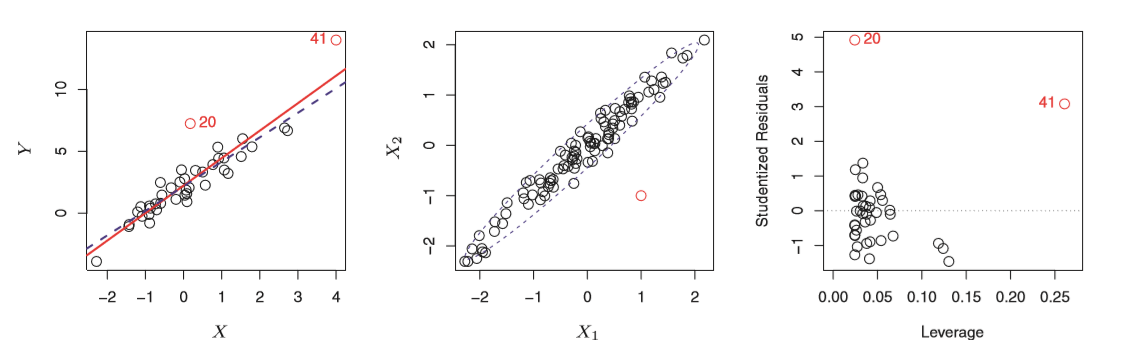
\includegraphics[width=\textwidth]{high_leverage.png}
    \caption{In this Fig. you see two outlying points ($20,41$), but only one of them ($41$) has a high leverage.}
    \label{fig:high_leverage_example}
\end{figure}

Furthermore, collinearity is an effect, that affects the accuracy of our previously mentioned $t$-statistic. To detect collinearity, we might want to have a look at the entries of the correlation matrix, but this is only possible in small dimensions. Even that, if more than two predictors are correlated we call that multicollinearity, which $\mathbf{cannot}$ be seen in the matrix. Here we assess the $\textit{variance inflation factor}$, which is one if no multicollinearity occurs. 
$$VIF(\hat \beta_j) = \frac{1}{1-R^2_{X_j|X_{-j}}}$$

where we have that $R^2_{X_j|X_{-j}}$ as the $R^2$-value for the regression of $X_j$ onto all the other predictors. So if $R^2$ is large we expect a higher collinearity.  


\newpage
\section{Chapter 4 - Classification}

As discussed before, we use the Classification setting if we have quantitative responses. Even though we could theoretically model the classification problem with the linear regression, there are subtleties that we want to avoid. In this case there are several different possible models to calculate our classification. What these are will be discussed when each is presented. \par
The problem with linear regression is the fact that we oppose an $order$ to our dummy variables. This indicates a difference between the outcomes, i.e. several classes. In order to be independent of the order, we need to use a classification setting/model. This problem gets severe if we have more than 2 classes, since we would have 2 differences between those classes. To conclude, in a binary setting, we can use the linear regression, else we use the classification setting. Yet there is still one problem with linear regression, and that is the fact that linear regression might predict probabilities that are less than $0$ or larger than $1$! Hence we use the following fitting approach.

\subsection{Logistic Regression}

We showcase a simple data-set, which indicates the advantages of the logistic model, it also shows it approximately works. 


\begin{figure}[ht]
    \centering
    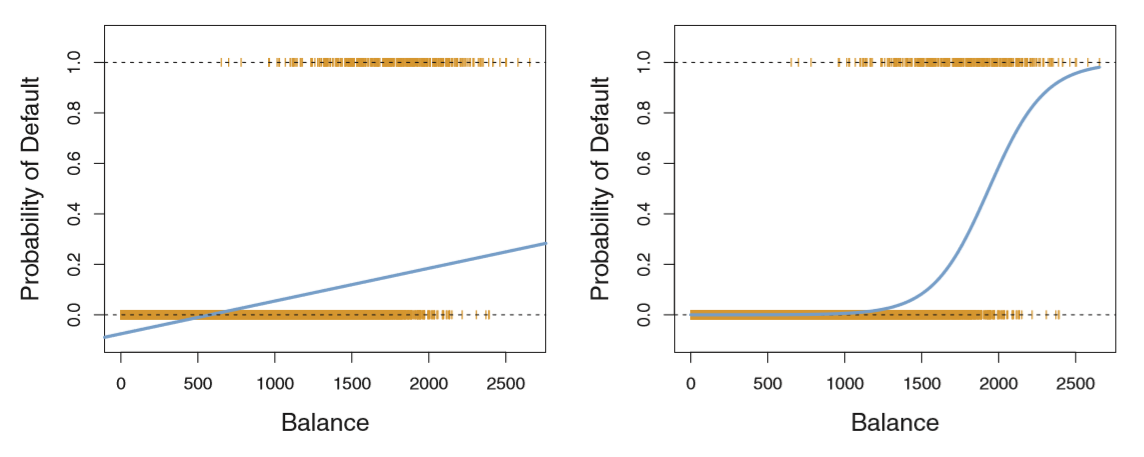
\includegraphics[width=\textwidth]{linear_logistic.png}
    \caption{In this set the data $default$, which is binary, is fitted over the $Balance$ predictor (see Textbook for the data-set). Hereby we see the problems with linear regression, so the logistic, on the right, is compared to it. We intuitively see that it is a better fit, especially for low $Balance$, it also fixes the probability problem that we had earlier.}
    \label{fig:linear_logistic_showcase}
\end{figure}

We can interpret this as $\mathbb{P}(\text{default}=\text{Yes}|\text{balance})$. \par

Recall the linear regression model, $p(X)=\beta_0+\beta_1X$, and as mention above, we wish to use a slightly modified model: 
\begin{equation}\label{eq:logistic_model}
    p(X) = \frac{e^{\beta_0+\beta_1X}}{1+e^{\beta_0+\beta_1X}}
\end{equation}
To fit it we use the maximum likelihood model, which will be shown later, but not fully discussed. With simple arithmetic manipulation of Eq.(\ref{eq:logistic_model}), we get:

\begin{equation}
  \log \Bigg{(} \frac{p(X)}{1-p(X)} \Bigg{)} =\beta_0+\beta_1X
\end{equation}
The left hand side is called $log-odds$ or $logit$, which is again linear in $\beta_1$. This has as a result, that the probability and our predictor are not linearly correlated.

Since the predictors $\beta_{0,1}$ are again unknown, they must be predicted using the training data, without other help. We try to find $\beta_{0,1}$, such that $p(\beta_{0,1})$ is as close to the data as possible. We use the $likelihood$ function:

\begin{equation}
    l(\beta_0,\beta_1)= \prod_{i:y_{i}=1}p(x_{i}) \prod_{i':y_{i'}=0}(1-p(x_{i'}))
\end{equation}

Now one chooses the predictors $\hat{\beta_i}$ to $maximise$ the likelihood function. The general setting how to calculate and explicitly compute the function, is another topic. Most statistical programs have algorithms to calculate a maximal $p(\hat{\beta_i})$. Yet we can still use $H_0$, the Null-Hypothesis, to evaluate the accuracy of our fit parameter.

\subsection{Multiple Logistic Regression}
Analogue to linear regression, we can use multiple predictors to calculate our model. Simply if we have more than one predictor this method is used. 

\begin{equation}
    p(X)=\frac{e^{\beta_0 + \sum_{i=1}^{p}\beta_{i}X_{i}}}{1+e^{\beta_0 + \sum_{i=1}^{p}\beta_{i}X_{i}}}
\end{equation}
Or alternatively the logit function,

\begin{equation}
    \log \Bigg{(} \frac{p(X)}{1-p(X)} \Bigg{)} = \beta_0 + \sum_{i=1}^{p}\beta_{i}X_{i}
\end{equation}

which was seen in a similar form in the multiple linear regression. 
There is a subtle important note for comparison between the simple classification and the multiple regression; there is a possibility that for the simple model the predictor is negative, but the $\mathbf{same}$ predictor in a multiple regression is positive. How is that possible? Let us consider the $default$ data again. For example one predictor might be student, and for the multiple one $balance, income$. In the simple case, $student$ is negatively correlated, meaning students are in general more likely to default, $\mathbf{but}$ if we consider the multiple case, and we consider individuals with the same income and same savings, students are $\mathbf{less}$ likely to default. This is especially important for interpretation later. \par

Theoretically this approach with the logistic regression is extendable to more than two classes, but this is not of a big concern here and the functions are available in most statistic packages. 

\subsection{Linear Discriminant Analysis}

There are several reasons why one might use the LDA method compared to logistic regression: 
If the classes are well separated logistic regression is unstable (meaning that a small variance in inputs might result in a huge difference in fit parameters) , similar case if $n$ is small and the points are approximately normal and LDA is in general more popular than linear regression for more than 2 classes.\par

LDA uses essentially Bayes' theorem. We define the prior function as $\pi_{k}$, which is essentially our guess for the classes or the probability, which are the proportions of the amopunt of classes in the sample for a random variable. Furthermore, we denote the $\textit{density function}$ as the following probability; $f_k=\mathbb{P}(X=x|Y=k)$, which is the density function for X having the class $k$. Generally it is difficult to calculate $f_{k}$, unless we do some assumptions. Thus Bayes' theorem states 

\begin{equation}\label{eq_bayes_LDA}
    \mathbb{P}(Y=k|X=x) = \frac{\pi_{k}f_{k}}{\sum_{j=1}^{K}\pi_{j}f_{j}}
\end{equation}
with $K$ as the amount of classes, where $\pi_k = \bP(Y = k)$.

\subsection{LDA | p=1}
For simplicity we consider one predictor now and we increase $p$ later. As mentioned above, one must make assumptions for $f_{k}$. For now we will assume normal distribution and make conclusions for that.
 Thus, 
 
\begin{equation}\label{eq_1D_normal_LDA_def}
    f_{k}= \frac{1}{\sqrt{2\pi}\sigma_k}exp \Bigg{(}\frac{-(x-\mu_k)^2}{2\sigma_k^2}  \Bigg{)}
\end{equation}
And according to Eq.~\eqref{eq_bayes_LDA}, we have for the probability

\begin{equation}\label{eq_normal_bayes_LDA}
    p_{k}(x) = \frac{\pi_{k}f_{k}}{\sum_{j=1}^{K}\pi_{j}f_{j}}  = \frac{\pi_{k}\frac{1}{\sqrt{2\pi}\sigma_k}exp \Big{(}\frac{-(x-\mu_k)^2}{2\sigma_k^2}  \Big{)}  }{\sum_{j=1}^K \pi_{j}  \frac{1}{\sqrt{2\pi}\sigma_j}exp \Big{(}\frac{-(x-\mu_j)^2}{2\sigma_j^2}  \Big{)}}
\end{equation}

For simplicity we also assume that $\sigma_k=\sigma$, for all $k$ in our observations. This it not necessary, but it simplifies most of it.
Since the denominator in Eq.~\eqref{eq_normal_bayes_LDA} is simply a constant, we can take the $\log$ of the Eq.~\eqref{eq_normal_bayes_LDA}, because it is monotonic, and we maximise the following;

\begin{equation}\label{eq_delta_bayes_1D}
  \delta_{k}=x \frac{\mu_k}{\sigma^2} - \frac{\mu_k^2}{2 \sigma^2} + \log(\pi_k)
\end{equation}

Even though we can guess the probability function we still need to calculate $\mu_i,\pi_i,\sigma^2$. The LDA approach uses the following assumptions:

\begin{equation}
    \hat{\mu} = \frac{1}{n_k}\sum_{i:y_i=k}x_i
\end{equation}

With $n_k$ being the number of members, and for our variance

\begin{equation}
    \hat{\sigma}^2 = \frac{1}{n-K} \sum_{k=1}^{K} \sum_{i:y_i=k} (x_i-\hat{\mu}_k)^2
\end{equation}

one can see that $\hat{\mu}$ is simply the average over all samples, and $\hat{\sigma}^2$ is the weighted variance over all classes. We might have a direct class membership probability $\pi_i$, but in absence of that information, we use $\hat{\pi}_k= n_k / n$.

\subsection{LDA: arbitrary p}

Obviously we would like to increase our predictors to multiple dimensions. Most of the theory still applies, with some continuation to higher dimensions.
First of all we need to update the $f_k$, so it is sufficient for higher $p$. We define it the following way:


\begin{equation}\label{eq_normal_pD_LDA_definition}
    f(x) = \frac{1}{\sqrt[p]{2\pi} \sqrt{|\mathbf{\Sigma}|}}exp \bigg{(} -\frac{1}{2} (x-\mu)_i \Sigma_{ij}^{-1} (x-\mu)_j  \bigg{)}
\end{equation}

Where we used that $X\sim \mathcal{N}(\mu,\mathbf{\Sigma})$, with the definition of multivariate normal distributions, so $\mathbf{\Sigma} = Cov(\mathbf{X})$. Note, that if let $p=1$ again we would have that Eq~$\ref{eq_normal_pD_LDA_definition}$ is equal to Eq~$\ref{eq_1D_normal_LDA_def}$, since $Cov(X) = \sigma ^ 2$ for one dimension. So for $k$ classes we would have that every class is distributed with $\mathcal{N}(\mu_k,\mathbf{\Sigma})$.
So for the Baye's classifier, assuming that we plug Eq~$\ref{eq_normal_pD_LDA_definition}$ into Eq~$\ref{eq_normal_bayes_LDA}$ and try to maximise $\delta_k$, we end up with 


\begin{equation}
    \delta_k = x_i \Sigma_{ij}^{-1} (\mu_{k})_j - \frac{1}{2} (\mu_{k})_i \Sigma_{ij}^{-1} (\mu_{k})_j + ln(\pi_k)
\end{equation}

Note, that it is the $p$-dimensional version of Eq~$\ref{eq_delta_bayes_1D}$, yet in the one-dimensional case it is still a scalar, because we still use the contraction between 2 vectors and a matrix($\mathbf{\Sigma}$).Also, we compute $\pi_k$, $\mu_k$ and $\mathbf{\Sigma}$ in a similar fashion as in the one-dimensional case. The decision boundary is once again calculated by computing $\delta_k = \delta_l$ between the $k$-th and $l$-th class. For applications it might be interesting to not place the decision boundary at $\mathbb{P}(default=Yes|X=x)>p$ for $p=0.5$ but let us say for $p=0.2$. This might again be interesting for the default case. So more individuals get correctly assigned the $default$ class, but it comes at a cost; now more people that do not default get classified as $default$. So again we have a trade-off between which error to minimise. Since this is dependent on the special case, we cannot generally say how to choose the boundary. \par

In general this is dependent on the so-called $\textit{domain knowledge}$, such as a cost if one assigns one to a certain class. For the $default$ example we have the following ROC($\textit{receiver operating characteristics}$) curve, which tells us this error for missed defaults.

\begin{figure}[ht]
    \centering
    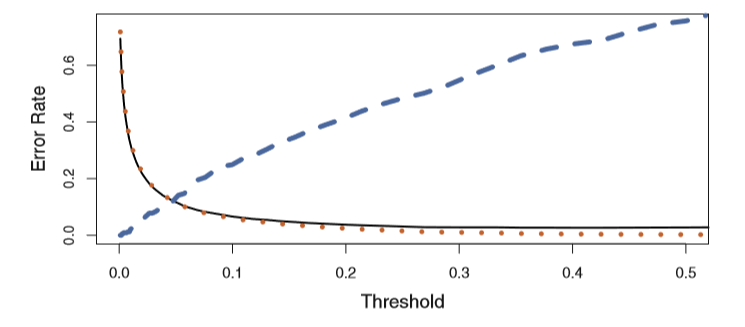
\includegraphics[width=\textwidth]{ROC_curve.png}
    \caption{the black line are the total errors, the orange error are the ones that did not $default$, but were wrongly assigned, and the blue points are the errors that did $default$, but were wrongly assigned. In this example one wishes to minimise the error rates for the blue line, while the total error rate does not go up too much. But people that $default$ that are wrongly assigned are bad for the credit card company that overlooks the $default$ data of it's customers}
    \label{fig:ROC_curve_example_default}
\end{figure}

Further reading is useful for explicit examples.

\subsection{Quadratic Discriminant Analysis - QDA}
This is a rather simple continuation for the LDA approach in higher dimensions. There we assumed that each measurement hat the same co-variance matrix $\mathbf{\Sigma}$, but now we assume each class has it's own co-variance matrix $\mathbf{\Sigma}$. Thus we have $X\sim \mathcal{N}(\mu,\mathbf{\Sigma}_k)$, which changes the definition for our $\delta_k$;

\begin{equation}
    \delta_k = -\frac{1}{2} (x-\mu_k)_i (\Sigma_{ij})^{-1}_k (x-\mu_k)_j -\frac{1}{2}\log(|\mathbf{\Sigma}|) +\log(\pi_k)
\end{equation}

and in explicit examples, one sees that the accuracy between LDA and QDA lies again in the bias-variance-trade-off. So for a linear model LDA (and similarly the logistic model) is slightly better, and for a more complex one then QDA approach might fit better. If it gets highly non-linear, one might consider the non-parametric KNN approach. A priori no one knows which model to use, unless you know the linearity of the model. In comparison to the linear regression, we have that the accuracy is dependent on the true distribution. If the decision boundary is linear, for which we choose LDA or logistic regression, moderately non-linear, QDA, or highly non-linear, KNN.
\newpage



\section{Resampling Methods}

Resampling is a method used in machine learning to obtain additional information from a given data set. As the name suggests, one takes several samples from the same test data to gain additional information. At first one does wonder how one gets additional information out of the data. But for example if one uses all data at once to fit, one obtains only one value for the variable, but if one splits the data into several sets, one might obtain several values. Thus one can obtain more information. The methods are represented here and applicable for most training methods. We will present cross-validation and bootstrap.

\subsection{Cross-Validation}

As we recall, calculating the training error is simple, but if one does not have the test results, the test error might be difficult to obtain. For a very large training set we might calculate it easier, but for a small given set it is more difficult. Here we take out a few observations and then fit the model without those data points. From that we might infer further information.

\subsubsection{Validation Set Approach}

The idea is simple; you split the data randomly into two sets, and train your model onto one set and test it with the other (this was also done in earlier lab problems). For quantitative problems one usually uses the MLE again for testing. Now for further accuracy one can repeat this process to recognise further trends. In general the MLE curves do not have to agree, only the general behaviour, i.e. like if a model; is linear or quadratic. However, there might be two disadvantages. First the validation MLE is not always consistent, meaning that it depends a lot on the selected validation set. Even though one can recognise trends, it is not accurate. Second the test is only trained on half the set, meaning that the modelling is dependent on a smaller subset. And in general greater subsets result in better fits.

\subsubsection{Leave-One-Out Cross-Validation}

This approach, called LOOCV, is similar to the previous one. But instead of taking half the set one just leaves out one data point, as the name suggests. What one calculates differs a bit:

\[
\text{MSE}_i = (y_i-\widetilde{y}_i)^2
\]
given the data point $y_i$ and the resulting fit without that point $\widetilde{y}_i$. This test error is very variable, since it is based on one point. So we repeat this procedure. The LOOCV estime is the normed sum of the errors, 

\[
\text{CV}_{(n)} = \frac{1}{n} \sum_{i=1}^n \text{MSE}_i.
\]

Some advantages are following. Less bias, due to the fact that we almost use all the data. Thus the test error does not get over estimated. Also there is less randomness in the training and validation sets, since every point will get used. \par
Disadvantage is the fact that it might get computationally heavy. But there is a
shortcut for linear models, where one can reduce the modelling of n  data-sets
to only one(!) data-set, proven in \cite{rob_j_hyndman_2014}:

\begin{equation}
    \text{CV}_{(n)} = \frac{1}{n} \sum_{i=1}^n \Bigg(
    \frac{y_i-\hat{y}_i}{1-h_i}
    \Bigg)^2.
\end{equation}

Here $\hat{y}_i$ (defined in previously) is the fit for all points, and $h_i$ is defined in~\eqref{eq:leverage}. This can be used for any kind of predictive modelling. 

\subsubsection{k-Fold Cross-Validation}

Now there is another option consisting of a combination of the previous ones. Instead of taking n data-points, one divides the data-set into k random sets. Similar to the LOOCV, one has for the CV estimate:

\[
\text{CV}_{(k)} = \frac{1}{k} \sum_{i=1}^k \text{MSE}_i,
\]
where the MSE are the corresponding test MSE of the divided sets. 

Why use this method? 
First, we have a computational advantage, since we do not need to fit the model n, but only k times, which is mostly between 5 and 10 (for $k=n$ we have again the LOOCV). Even though we have a variability in the CV, it is not as high as in the validation approach. And even though it might seem completely different, LOOCV and k-fold cross validation produces similar test MSE values, which is important to find the best flexibility for our model. \par

As mentioned before, there is for most models a variance-bias trade-off. 
Here the k-fold validation has a higher bias, since it has less observations. But because one uses several data-points multiple times, the fitted models are highly correlated, making the LOOCV have a higher variance. Thus one chooses k to be between 5 and 10 for most of the times. 

\subsubsection{Cross Validation for Classification Problems}
The previous methods were for quantitative regressions, but we would like to generalise for classifications setting. 


\[
\text{CV}_{(k)} = \frac{1}{k} \sum_{i=1}^k \text{Err}_i,
\]
where $ \text{Err}_i=I(y_i\neq \hat{y}_1)$, and the other methods defined analogously. Similar to the previous methods, we use this to decide for the fit of model. 


\subsection{Bootstrap}

In general bootstrap is a widely used method for estimating standard errors. Even though most packages can do that for linear regression, this can be used for a variety of models. 
Suppose we wish to invest a fixed amount of money in different assets X and Y, for which we allot $\alpha$ to X and $1-\alpha$ to Y, and in order to minimise risk, we want the variance to be minimal. 
Hence minimise Var($\alpha$X + (1-$\alpha$)Y), and it can be shown that

\[
\alpha = \frac{\sigma_Y^2 - \sigma_{XY}}{\sigma_X^2+\sigma_Y^2 - 2\sigma_{XY}}.
\]
Again, since we do not know the actual variances, we calculate $\hat{\alpha}$ instead of the true value. So how do we get new samples from our data? Instead of gaining sets from the population or experiment, we draw new samples from the original data set! Here we draw from the data with replacement, call it $Z^{*1}$, and from that we calculate the $\alpha^{*}_1$. In total we draw B estimates of the data, and our estimate for the standard error of $\alpha$ is 

\begin{equation}
    \text{Var}_B(\alpha) = \frac{1}{B-1} \sum_{i=1}^B(\alpha^{*}_i - \overline{\alpha ^{*}_B})^2
\end{equation}
\newpage

\section{Linear Model Selection and Regularisation}

As seen in the linear regression setting, we have an outcome $Y$, that is dependent of several predictors $X_i$. Usually one uses the least squares fit for the regression. However one wants to possibly improve the least squares fit, for alternative methods for special cases. Different methods yield sometimes better interpretability and better accuracy. 

The accuracy is worse for least squares for cases when $n$ is not large compared to $p$, one might over-fit, resulting in bad variance. Even worse if $p$ is larger than $n$ there are infinitely good fits with zero least squares. In practice this usually happens for experiments where one has only a few measurements but loads of predictors. 

The predictability suffers from the fact that some predictors have no influence in the actual event or mechanism. Those predictors are irrelevant, but in least squares it is unlikely to be exactly zero. So one needs to find a method to set them exactly to zero.

To summarise the alternatives, one has Subset selection, where one chooses predictors that are actually relevant. This was already mentioned before, but we will explore this furthermore. Shrinkage is the method in which we use least squares but the ones that are relatively close to zero get shrinked to zero. This method reduces variance, since unnecessary variables do not interfere with the test MSE. Another one is dimensional reduction, in which one reduces the $p$ predictors to $M$ dimensions. One projects the variables onto a smaller subspace.  


\subsection{Subset Selection}
\subsubsection{Best Subset Selection}
As the name suggests, one chooses the best subset of all possible predictors. For $p$ predictors for each step we choose $k$ predictors, so we have to fit the model ${\binom{p}{k}}$ times, and in total $2^p$ times. Choose according to the prediction of errors. So for each step we have a best model, and out of all of them we have to choose the very best. Do that according to bias-variance-trade-off. This obviously becomes very computationally heavy, for large $p$. So computationally if $p>40$, then we have to choose different methods. 

\subsubsection{Stepwise Selection}
A computational efficient alternative is the stepwise selection. 

Forward selection, where we start with a null-model, with no predictors. Consequently add new predictors with the best fit, according to previous estimation methods. So consecutively we add single predictors, until we have $p$ different models. Out of these choose again the best, according to previous chapters. So following this algorithm we have $\sum_{k=0}^{p-1}(p-k)=1+\frac{1}{2}p(p+1)$. Advantage is computationally, but the disadvantage is that we are not guaranteed to find the best model. This can be even applied for high dimensional $p$, but only on a subset of maximal $n$ predictors.

Backward selection can be done the same way, except that one starts with a model of full predictors and then slowly reducing the predictors until one finds the best model. It has the same order of complexity, compared to the forward selection. Also if $p>n$ we cannot start with a model with full predictors, given we use least squared method.

We can also combine these two, starting with arbitrary amounts of predictors and then add or subtract new predictors. This might come closer to the true best subset. Then again this might become computationally heavy again.


\subsubsection{Choosing the Optimal Model}

The previous methods are only useful if we can estimate the actual test error and not the training error. Thus we could either use the direct estimation of the cross validation, or we make adjustments to the training errors. 
We recall that the training MSE is generally lower than the test MSE, so we can seek adjustments if we increase the MSE if once chooses to increase the used predictors.

The first to consider is $C_p$, if one fits with the least squares methods (so one can obtain the standard error).

\begin{equation}
C_p = \frac{1}{n}(RSS+2p\hat{\sigma}^2),
\end{equation}
where $\hat{\sigma}$ is the estimate of the standard error, given in previous chapters (confer to the Bayes' estimators). One can show that if $\hat{\sigma}$ is an unbiased estimator of $\sigma$ then $C_p$ is an unbiased estimator of the rest MSE \cite{degroot2013probability}. As a result we can estimate the test error. 

The next one is $\text{Akaike Information Criterion}$, which is defined for a general set of functions. Let p be the amount of predictors and $\hat{L}$ the maximum value of the likelihood function (defined earlier), then we have:
\begin{equation}
    AIC = 2p -2\log (\hat{L}),
\end{equation}
which is at first a complicated definition, but in the Gauss case, we have that $C_p \propto AIC$, so we can more or less ignore it for now. 

The bayesian information criterion (BIC), is defined as follows:

\begin{equation}
    \text{BIC} = \frac{1}{n\hat{\sigma}^2} (\text{RSS} + \log(n) p \hat{\sigma}^2).
\end{equation}
As in previous examples we select the model with the lowest test error, hence the lowest BIC. Since $\log(n)>2$ for $n>7$, we have that for large samples, that the BIC sets a higher penalty for many variables. 

The adjusted $R^2$ places again a penalty for many variables, since $R^2$ would be increasing monotonously instead. 

\begin{equation}
    R^2_{adjusted} = 1- \frac{\text{RSS} (n-1)}{\text{TSS} (n-p-1)}.
\end{equation}
 To find the maximum of that is to find the minimum of $\frac{RSS}{n-p-1}$. So this is motivated in that sense that if one increases $p$, one decreases the adjusted $R^2$. So we have another estimation of how to find the test MSE.
 
\subsection{Shrinkage Methods}
 Instead of trying to find a perfect model, we could instead start with the full model and try to shrink it. Hence the non-necessary parameters will be shrunk to zero. In some cases this might become computationally more easy. We will consider lasso and ridge regression. For this section we need a bit of functional analysis. For that we define the $p$-Norm as the following:
 
 \begin{equation}
     \|x\|_p^p = \sum_{i=1}^n |x_i|^p  \quad \text{for $1 \leq p \leq \infty$}.
 \end{equation}
 
Furthermore we recall the Lagrange formalism for multipliers. We only refer to
the theorem and we cite the proof (\cite[page 414]{marsden1993elementary}):

\begin{equation}
    \nabla f(x_0) = \lambda ^* \nabla g(x_0),
\end{equation}
 with the constraint $g(x_0)=s$ and the Lagrange multiplier $\lambda ^*$ (not to confuse the parameter listed below). With $f|S$ (constrain of the manifold) and $S=g^{-1}(s)$ (definition of the manifold). 
 
 \subsubsection{Ridge Regression}
 If we recall how one defined RSS, we can tweak it by the following way:
 
\begin{equation}
     \text{RSS}_{ridge} =  \sum _ {i=1}^n (y_i-\hat{y}_i)^2 + \lambda \sum_{i=1}^p \beta_i^2 = \text{RSS} + \lambda \sum_{i=1}^p \beta_i^2.
\end{equation}
 Whereas $\lambda \geqslant 0$ is a tuning parameter, which is to be determined later. So similar to before one tries to minimise RSS. But now we have a penalty for parameters, meaning that the $\hat{\beta}_i^R$ get shrunk more towards zero. So parameters that do not contribute to a large shrinking of RSS result in a higher ridge parameter, due to the penalty. 
 For low $\lambda$ we have a least square fit, for $\lambda \to \infty$ we will receive the null hypothesis $H_0$.
 As a connection to functional analysis, $\sum_{i=1}^p \beta_i^2. = ||\beta||_{2}^2$ as the $\ell_2$-Norm. We divide each $\beta$ by its vector norm to compare different fit parameters. Just because many scales are dependent of the factor normalising it prevents errors. 
 
 So why do we use this method?
 First of all it is a generalisation, meaning that in the end we might receive the least square fit again if we wish to. In essence, the advantage is again the variance-bias trad-off. If we increase $\lambda$, the variance decreases, since the parameters get shrunk further to zero. But for decreasing $\lambda$ the bias increases. So in total we would have a minimum for the test MSE,to minimise both errors. If the data is close to linear we have a high variance for least squares. Since ridge regression can trade off high variance for low bias, it performs better than least squares for data with high variance. Also we do not have to work through $2^p$ models, instead we only need to fit one model and we can fit $\lambda$ simultaneously for arbitrary values. This is then computationally better.
 
 \subsubsection{The Lasso}
 The disadvantage of the ridge regression is the fact that we shrink the predictors, but we never set them to zero. So the lasso method is better in the fact that it actually can set some predictors to zero. But before explaining how that works let's look into the method first. Considering that we used the $\ell_2$ Norm one might expect to use the $\ell_1$ Norm. This form is then the lasso method:
 
 \begin{equation}
     \text{RSS}_{lasso} = \sum _ {i=1}^n (y_i-\hat{y}_i)^2 +\lambda \sum_{i=1}^p  \beta_i =  \text{RSS} + \lambda \sum_{i=1}^p \beta_i,
 \end{equation}
whereas we have that the coefficients $\hat{\beta}_\lambda^L$ minimise the adjusted lasso RSS. Because the lasso forces some parameters to be zero (for sufficiently high $\lambda$), we also have a model selection in this method. This results in the fact that we can have less than p predictors.

But now back to the question to why the lasso does selection. This has to do with the fact how the unit sphere of both norms looks like. For $\ell_2$ we have a sphere, but for $\ell_1$ we have a diamond shape (this can be generalised).

\begin{figure}[ht]
    \centering
    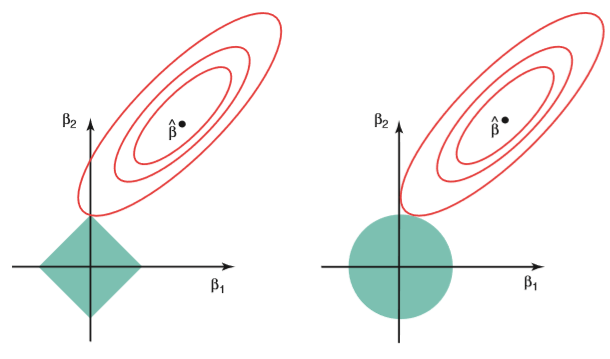
\includegraphics[height=70mm]{l1_l2_comparison.png}
    \caption{The blue areas are the (unit) spheres of the $\ell$ Norms (1 on the left, 2 on the right). The red ellipses are the contours of RSS.}
    \label{fig:comparing_l_norms}
\end{figure}

In the figure one can see that the intercept for $\ell_1$ is at 0 for some variables, whereas for the $\ell_2$ norm it is not (this might indicate a further selection for a norm $p<1$. But sadly in that case we do not have a norm. However we still could use it for estimation). 
 
 So which method to use?
 It is clear that the lasso has the advantage of setting some predictors to zero. This is useful if one wants to interpret the predictors. However there is more to consider. If we have many useful predictors, almost all p of them, then we do not want to set some of them to zero. However if only 2 of dozens of predictors are important we definitely want to set them to zero. So in general the ridge regression might reduce variance, whereas the lasso is easier to interpret. Hence the better fit is dependent on the data set. Again we can make use of the cross validation to choose the model. 
 
 
 \subsubsection{Bayesian Interpretation}
 Recall lecture for prior and posterior distribution, with $p(\beta|X,Y) \propto
 f(Y|X,\beta)p(\beta)$ (posterior is proportional to likelihood function times prior  \cite{degroot2013probability}.
So with the prior as $p(\beta) = \Pi _{i=1}^p g(\beta_i)$ with g as a density function. We find that the density functions for lasso and ridge are the following: 

If g is a Gaussian distribution with mean zero and standard deviation of $\lambda$, one has for the posterior mode for $\beta$ that is is given by the ridge regression. Also the ridge regression is the posterior mode.

If g is a double exponential or Laplacian with mean zero and parameter $\lambda$, one finds for the posterior mode the lasso regression. Also the same process for the posterior distribution.

Hence the ridge assumes that parameters are normally distributed around zero, whereas the lasso assumes some parameters to be zero.

\subsubsection{Selecting the Tuning Parameter}
 As discussed earlier we can estimate performance by cross validation. First we choose a grid for $\lambda$ and then we choose the best one according to the cross validation for the specific data set. Then we use this parameter and do the corresponding fit, either ridge or lasso method. So generally we cannot say a lot about this algorithm, if we do not have more information about the data.
 
 
 \subsection{Dimension Reduction}
 As the name suggests, with this method we reduce (or in general change) the dimension of our predictors. So going from p predictors we change to M predictors by:
 
 \begin{equation}
     Z_m = \sum_{m=1}^p \phi_{jm}Xj,
 \end{equation}
 for the predictors $X_j$ and some constants $\phi_{jm}$ that represent a linear transformation (that has to be chosen). So with the new $Z_i$ we fit those with previous models. Of course we need to consider how to choose the parameters $\phi_{jm}$.
 
 \subsubsection{Principal Components Analysis}
 
 We define this here a bit more mathematical than in the book. The PCA is the following orthogonal transformation. The projection of the data with the greatest variance gets sent to the first transformed coordinate. The following coordinates. The second largest variance of a possible projection (orthogonal to the first one) gets sent to the second coordinate, and so on. It turns out that this method for fitting is useful if only a predictors are needed for the model. That said PCA and ridge regression are alike in the sense that ridge regression is a continuous case of the PCA (\cite{hastie01statisticallearning}). Again we choose the number of dimensions M by cross validation. As before standardising the parameters is recommended for comparison of other methods or unit systems. If we subtract the mean column of the Matrix $M$ we have $\widetilde{M}$. We define the principal components as the eigen-vectors of $C=\widetilde{M}^* \widetilde{M}$. To look what this means let us analyse M. It is the matrix defined as $M=x_{ij}$ for $i\in [1,n]$ and $j\in[1,p]$ as the values of the $i$-th data-point for the $j$-th predictor. Thus $\widetilde{M}= (x_{ij}-\bar{x}_j)$. Hence
 
 \begin{equation}
     C= \widetilde{M}^* \widetilde{M} = \sum_{i=1}^n(x_{ki}-\bar{x}_k^T)(x_{ij}-\bar{x}_j)=Corr(X,X),
 \end{equation}
 which is the definition of the correlation matrix.
 However this method has a problem in the sense that we still end up with all p predictors, only in a smaller dimension. Hence interpretability suffers. Also noise parameters, also predictors that do not contribute, are included in PCA (see also ridge regression).
 Considering information theory, the more variance a variable it has, the more information it carries. For that reason we would like to find the eigenvalues with the highest variances. This makes it less likely to interpret, but we reduce the dimensions massively. Technically speaking we still have the same dimensions, but we can ignore the ones with low variances.
 
 \subsubsection{Singular Value Decomposition}

 Suppose we have a $m \times n$ data matrix M, then we can decompose M in following matrices:
 \begin{equation}
     M = U \Sigma V^*,
 \end{equation}
 with U being a $m \times m$ unitary matrix, V (and it's transposed [conjugated] $\text{V}^*$) a $n \times n$ unitary matrix and $\Sigma$ a diagonal matrix with non-negative numbers $\sigma_i$. Note for $n \neq m$ U and V are not uniquely defined. $\Sigma$ however is always unique. In the case $n=m$ we have unique U and V (they are in fact equal), since that case is the standard diagonalisation process. 
 
 In the data sense $\text{U}_i$ is the $i^{th}$ eigen-sample, and $\text{V}_i$ is the $i^{th}$ eigen-feature. So the normalised diagonal components $\sigma_i / ||\sigma||_2$ correspond to the percentile variances. 
 
 Now if we compare both $\widetilde{ M} =\widetilde{ U} \widetilde{\Sigma} \widetilde{V}^*$ so we have that for $C=\widetilde{M}^* \widetilde{M} =\widetilde{ V} \widetilde{\Sigma}^2 \widetilde{V}^* $.

\subsection{High Dimensions}

We noted before that data with predictors close to the data set number n can be problematic with least squares due to over-fitting. This problem becomes more relevant if the amount of predictors is even bigger than the data set. In practice this might arise from the fact, for example in genetics, that we want to model some phenological traits, while we have several thousand genomes in consideration. 

The problem in this case is that we have too much flexibility that does not really represent the causation effect. Thus we need alternative methods for fitting the high dimensional data.

It turns out that the previously discussed methods are able to reduce variance enough so that the $\lambda$ is restrictive enough to find the actual associated responses. So in general high dimensional data is double edged: new technologies are able to find new associations in predictors and data. Disadvantage is that many of those predictors are nothing but noise. Hence we need to be extra careful with this data. 

With the interpretation we need to be more careful as well. The more predictors the higher multicollinearity is. Thus we can most likely not identify the best variables. In practice this does not mean the model we found is useless. Yet it might mean that we cannot say for sure that the used predictors are the only possible ones decent enough for a fit. Also errors that are dependent on the least squares fit (see earlier) are useless, since the MSE equals zero. So to estimate test MSe we once again need to use cross validation as an estimate. This is not dependent on the fact that the least squares method works. 

\newpage
\section{Tree Based Methods}
\subsection{Basics for Regression Trees}
This methods splits up the sample space in different sections. The decisions how to split the data can be represented in a tree. The decision boundary can be plastered with different rectangles, or even more simple subsections. But how do we partition the sample space? For quantitative data we choose to have $R_1,\dots,R_J$ different partitions. Again we choose to minimise the RSS:

$$ \text{RSS}=\sum_{j=1}^J \sum_{i \in R_j} (y_i-\hat{y}_{R_j})^2. $$

the estimation of the rectangle $R_j$ is the average of all data in that separation, and 
$\hat{y}$ is the mean of all data points in this specific rectangle. Since finding the very best selections is computationally unfeasible, we do the following approach. We call it the greedy approach, because we start with one rectangle and then we successively start splitting it. This is greedy because that does not guarantee the best tree. Refer this problem to the previous subset selection problem. We select the split which has the lowest possible RSS. This process is continued until we reach a defined termination point.

\subsubsection{Pruning}

Pruning is the method of shrinking the tree. The greedy model most likely over-fits. We add a penalty for having too many ends, or nodes. Similar to the lasso we try to minimise

\begin{equation}
    \text{RSS}_{pruning}=\sum_{m=1}^{|T|} \sum_{i \in R_n} (y_i-\hat{y}_{R_m})^2 + \alpha |T|,
\end{equation}

with $|T|$ as the amount of terminal nodes, $R_m$ corresponding to the $m$th terminal node. Again we can choose $\alpha$ by getting the lowest cross validation error. The bigger the tuning parameter the less leaves we have.  

\subsubsection{Classification Trees}

With a simple tweak we can transfer this model into the classification setting. We assign a point to the class with the most occurrences. The corresponding error is the amount of points that do not belong into the largest class. We define the proportion $\hat{p}_{mk}$  of the $k$th class in the $m$th region. 

We define the Gini index as 

\begin{equation}\label{Gini_index}
    G= \sum_{k=1}^K \hat{p}_{mk} (1-\hat{p}_{mk}).
\end{equation}
It is easy to see that the Gini index is small if $\hat{p}_{mk}$ is close to zero or one. The resulting function is a concave parabola, with zeros at 0 and 1. Hence a small value indicates that node is relatively pure, which is useful later. 

We define the entropy as

\begin{equation}\label{entropy_tree}
    D=-\sum_{k=1}^K \hat{p}_{mk} \log \hat{p}_{mk}.
\end{equation}

This function appears more often in other parts of statistics and information theory. Similarly it is small if $\hat{p}_{mk}$ is close to 0 or 1. 

\subsubsection{Advantages and Disadvantages}

Again, if the model is linear, the linear model performs quite well. Is the actual model more compartmentalised, the tree model performs better. Also we have other aspects. Tree models are fairly easy to explain, and it mirrors more human based decision making (making it more applicable in real life). Trees can be portrayed easily, even in higher dimensions. The downside is that most trees are not as accurate, and they tend to be not robust (i.e. high variance). 

Hence we like to reduce those disadvantages.

\subsection{Improvements}
\subsubsection{Bagging}

Bagging is the term if we apply the bootstrap method for the decision trees. We define the bagging model as 


\begin{equation}
    \Hat{f}_{bag}(x)= \frac{1}{B} \sum_{b=1}^B \hat{f}^{*b}(x),
\end{equation}
if we take B bagging models $\hat{f}^{*b}$. Theoretically this can be extended for classification problems.

Furthermore, we can estimate the error with the out-of-the-bag (OOB) estimation. This is essentially the LOOCV method for the decision trees. However bagging comes at the cost of interpretability again. Yet we are able to measure which variables are important. This can be done by measuring how much one variable the RSS reduces.

\subsubsection{Random Forest}

This method decreases the correlation between the trees. In the previous method we still have a high correlation in these trees. Similar to bagging, we choose a number of samples. But when doing these trees we only allow a subset (m) of the predictors (p) instead of all of them. First this sounds weird. But in the previous example we always choose the most important variable. This would lead to an increased variance, since all tree models would include this variable. Hence in $(p-m)$ splits we do not have the important variable. This method is more specific than bagging, since we end up with in for $p=m$ again. This method turns out to be very useful with many highly correlated predictors, e.g. in biology.

\subsubsection{Boosting}

Instead of fitting the data directly to the predictors and the outcome, we let the tree slowly 'learn'. Given a tree, we improve that tree with the residuals and incrementally improve the worse prediction areas. We update the tree and the residuals. After the update we repeat the process. The algorithm goes like this:

set $\hat{f}=0$ and $r_i=y_i$ for all i in the training set. For b in B(number of trees) repeat: fit a tree $\hat{f}^b$ with d splits to the training data. Update the tree with the tuning parameter $\lambda$ and the residuals 

\begin{gather}
    \hat{f}_{new}(x) = \hat{f}(x)+ \lambda \hat{f}^b(x) \\
    (r_i)_{new}=r_i - \lambda \hat{f}^b (x_i).
\end{gather}
After we went through all the different added models we have for the final model:

\begin{equation}
    \hat{f}(x) = \lambda \sum _{b=1}^B \hat{f}^b(x)
\end{equation}

\newpage

\section{Support Vector Machines}
\subsection{Maximal Margin Classifier}
Fir, we need to define what a hyper-plane is. In $\mathbb{R}^n$ we have a $n-1$ dimensional hyper-plane as a flat affine subspace. So the hyper-plane is a $\mathbb{R}^{n-1}$ vector space. The hyper-plane is spanned by a orthogonal vector and a starting point. Every plane has a definition in parameters: 
\begin{equation}\label{marginal_classifier}
    \beta_0+\sum_{i=1}^n \beta_i X_i = 0.
\end{equation}
 
This is the equation for the plane being orthogonal to the plane vector (refer to the null space in linear algebra) 
This is quite suggestive for two reasons. This plane divides points into two regions, one for positive value for the sum in  \eqref{marginal_classifier}, one for negative values. The next is that our predictors span the plane for the said equation.

If the data is separated enough, this plane can split the data-sets. But then different planes split the data equally. That's why we need to introduce another condition.

This condition is called the maximal margin classifier, in which each point is the furthers away from the plane as possible.  

\begin{figure}[ht]
    \centering
    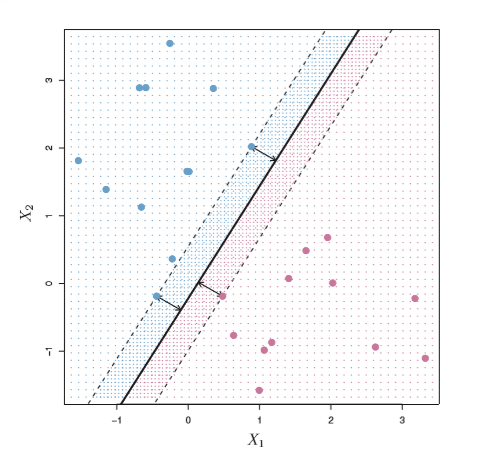
\includegraphics[height=70mm]{maximal_margin.png}
    \caption{In this figure you the the dividing hyper-plane. The two points in the blue and the red point define the plane. These are called the support vectors. }
    \label{maximal_margin}
\end{figure}
 
We already see that this plane in Fig \ref{maximal_margin} is dependent on these support vectors. This will be improved later.

The calculation of this plane equates to: 
\begin{align}
& \underset{\beta_i,M}{\text{Maximise}} M,\\
& \text{subject to} \\
&y_i(\beta_0+\sum_{i=1}^n \beta_i X_i )\geq M,\\
&\sum_{i=1}^n \beta_i X_i = 1.\\
\end{align}
for the observations $x_i \in \mathbb{R}^p$ and class labels $y_i \in {-1,1}$. As noted before, this solely works for separated classes. 

\subsection{Support Vector Classifiers}
The problems with the previous setting are the following: The planes are only dependent on the support vectors, making it unstable. Also we are not guaranteed a definite fit for the plane. We lift the strict restriction of having all points classified correctly. We optimise the following: 

\begin{align}
& \underset{\beta_i,M}{\text{Maximise}} M,\\
& \text{subject to} \\
&y_i(\beta_0+\sum_{i=1}^n \beta_i X_i )\geq M(1-\epsilon_i), \label{line_eq_support}\\
&\sum_{i=1}^n \beta_i X_i = 1\\
&\epsilon_i \geq 0, \quad \sum_{i=1}^n\epsilon_i \leq C.\\
\end{align}

Practically, the C is a tuning parameter calculates how many violations of the maximal margin classifiers there are. These violations are that some points are closer than the actual M. The bigger the C, the more violations there are. 

\begin{figure}[ht]
    \centering
    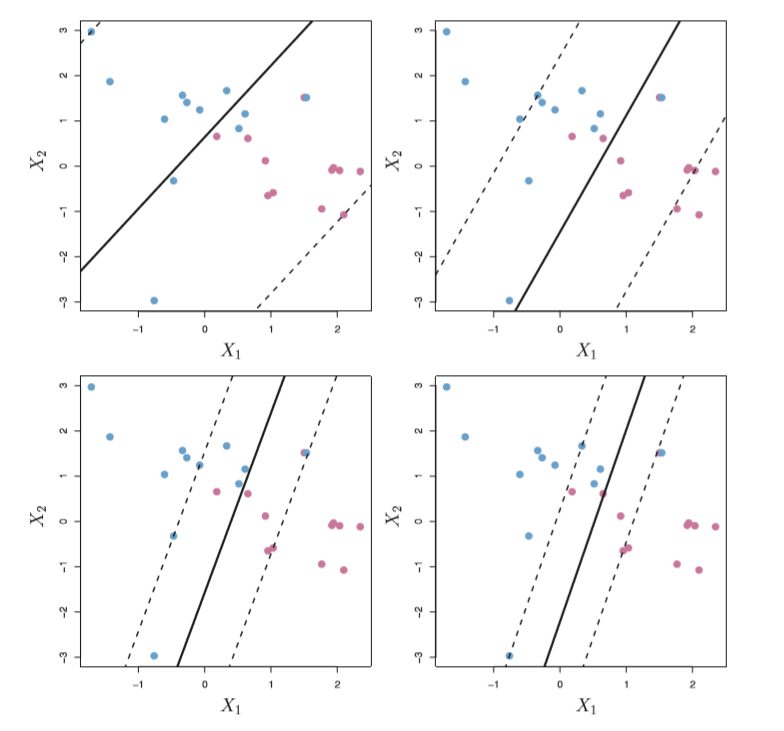
\includegraphics[height=80mm]{support_vector_classifier.png}
    \caption{The support vector hyper-plane for different values of C. Note that the direction of the plane changes for different values of C}
    \label{support_vector_classifier}
\end{figure}
In general, C is again dependent on the bias-variance trade-off. For higher C more support vectors are involved, hence a low variance. On the contrary for low values of C the bias is low as well. In Fig \ref{support_vector_classifier} we see examples for different classifiers. 

This optimisation is again containing the previous one (for $C=0$). But we still run into some issues. For simple reasons if we have boundaries that are not linear the hyper-plane will fail. Also there are examples with linear boundaries that fail as well. For example if class 1 is in between two heaps of class 2, where one simple hyper-plane cannot separate those two. 

\subsection{Support Vector Machine}

First we address the problem how to come up with non-linear boundaries. So instead of fitting linear combinations as in \eqref{line_eq_support}, we add some polynomial terms for the predictors. This is akin to previous sections, when we came from linear models to polynomials. 

\begin{figure}[ht!]
    \centering
    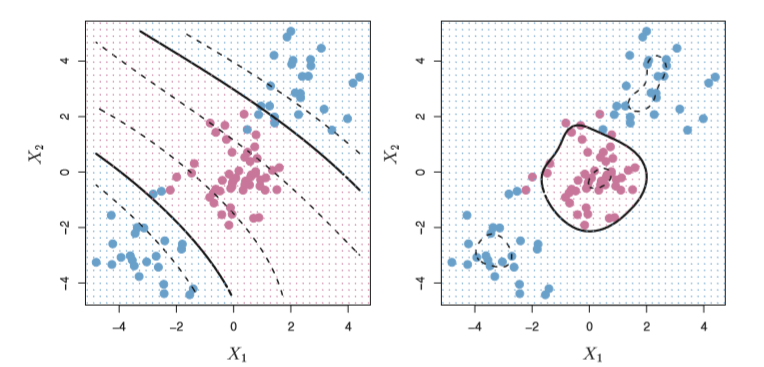
\includegraphics[width=\textwidth]{support_vector_machine_kernel.png}
    \caption{On the left the data is represented in a polynomial kernel. On the right with a radial kernel. One can see that the problem of the separation is solved by this method. Yet it is not clear which of those two perform better than the other.}
    \label{figure_SVM_new_kernel}
\end{figure}

We can generalise this concept. We define the inner product

\begin{equation}\label{inner_product_def}
    \langle a,b \rangle = \sum_{i=1}^n \sum_{j=1}^n a_i \eta_{ij} b_j,
\end{equation}
for some vectors a and b, and the corresponding metric $\eta$, which is simply the identity matrix in most cases. Hence the support vector machine classifier is defined as

\begin{equation}
    f(\mathbf{x}) = \beta_0 + \sum_{i=1}^n \alpha_i  \langle \mathbf{x},x_i \rangle. 
\end{equation}

We can replace \eqref{inner_product_def}, by a general function K, called the kernel. We simply define $K(x_i,x_j)$ as a general function. The inner product is a specific case of the kernel.

We present different useful kernels. The first one is the polynomial kernel.

\begin{equation}
    K(x_i,x_j) = (1+ \sum_{k=1}^p x_{ik}x_{jk} )^d,
\end{equation}

for some parameter d, or the exponential kernel with

\begin{equation}
     K(x_i,x_j) = exp (-\gamma \sum_{k=1}^n(x_{ik}-x_{jk})^2).
\end{equation}

\subsection{More Than 2 Classes}

The extension to more than 2 classes is not canonical. Yet it might be interesting to mention them. In the first one we compare each of the classes to each other. This is called one to one classification. After we finished the $\binom{K}{2}$ for the K classes, and we compare each point to which it was assigned the most. Similar to the majority vote in the previous chapter.

In the one versus all approach we fit one class of the $K$ classes to the rest of the $K-1$ classes. Then we assign a point to the class, for which $f(x)$ was the largest. 

However if we wish to actually program this algorithm we need to consider more than just the things stated. 


\newpage
\bibliographystyle{alpha}
\bibliography{references}
\end{document}